%% generated by make_results_tex.py
\subsection{Autonomous run in a home}
The robot was placed in a carpeted hallway of a furnished apartment at night with the room lights on, the exploration service was started from the PC and Explore was pressed once; nobody touched the robot or the keyboard afterwards. Doors stood as they were left; there are no stairs on this floor. \Cref{tab:run} summarises the run, \cref{fig:runmap} shows the saved map with the path the robot chose and \cref{fig:progress} the mapped area over time. Of the 30 goals sent, 24 were reached and 5 were cancelled because the frontier behind them was seen on the way; 1 failed (timeout after 156 s). Mapped area grows fastest in the first two minutes, when every goal opens a new room to the 360\textdegree{} lidar, and creeps up afterwards as the robot visits the corners and gaps behind furniture one at a time; the number of open frontiers peaks at about four and a half minutes and falls to zero after 11.6 minutes, when the robot returned to its start. The single failure was a goal on the far side of a wall that the planner could reach only through unknown space; the controller made progress but not enough, and the goal was dropped after its timeout of 156\,s. The mean speed over the run, 0.098\,m/s, is close to the controller's cruise speed of 0.10\,m/s, so the time was spent driving rather than waiting or recovering. The long white streak at the top of the map is free space seen along a few rays through a narrow gap (most likely a door left ajar); the frontier at its end is a ray or two wide, below the 0.30\,m minimum frontier length, so the explorer ignored it, which is also why the room behind it is missing from the map.

\begin{table}[t]
\centering\small
\caption{The autonomous run, from the explorer's log.}\label{tab:run}
\begin{tabular}{@{}lr@{}}
\toprule
Duration (start to end) & 12.6 min \\
Mapped area (known cells) & 47.3 m$^2$ \\
Free / occupied area in the saved map & 37.5 / 9.8 m$^2$ \\
Map extent & 10.9 $\times$ 13.2 m \\
Path length (SLAM poses, 5\,cm steps) & 74.0 m \\
Mean speed over the run & 0.098 m/s \\
Frontier goals sent & 30 \\
\quad reached & 24 \\
\quad seen on the way (cancelled) & 5 \\
\quad failed (blacklisted) & 1 \\
Operator interventions & 0 \\
Frontier search on the Pi, mean / max & 50 / 58 ms \\
Candidate frontiers per search, mean & 11.1 \\
Mapping rate & 3.8 m$^2$/min \\
Battery, start / end & 7.40 / 7.08 V \\
How it ended & back at the start \\
\bottomrule
\end{tabular}
\end{table}

\begin{figure}[t]
\centering
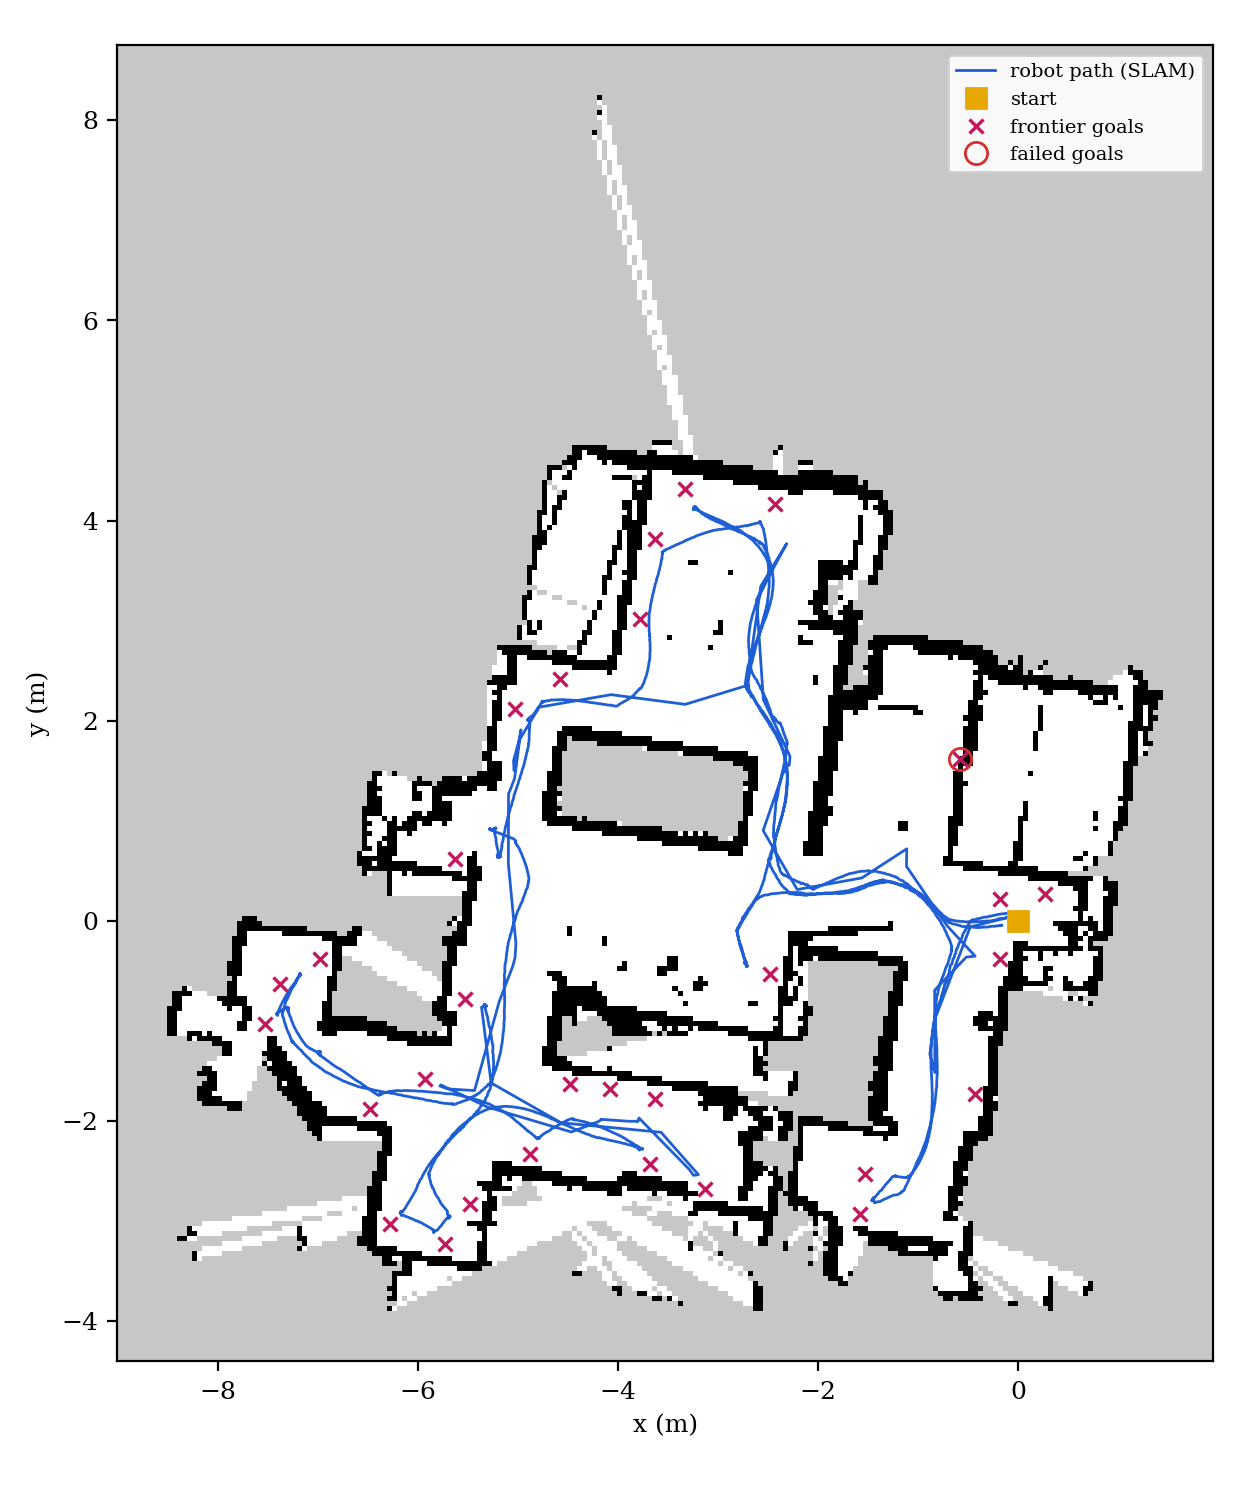
\includegraphics[width=\columnwidth]{figures/run_map.png}
\caption{Map saved at the end of the autonomous run (5\,cm cells; white free, black occupied, grey unknown), with the robot's path from SLAM, its start and the frontier goals it chose.}\label{fig:runmap}
\end{figure}

\begin{figure}[t]
\centering
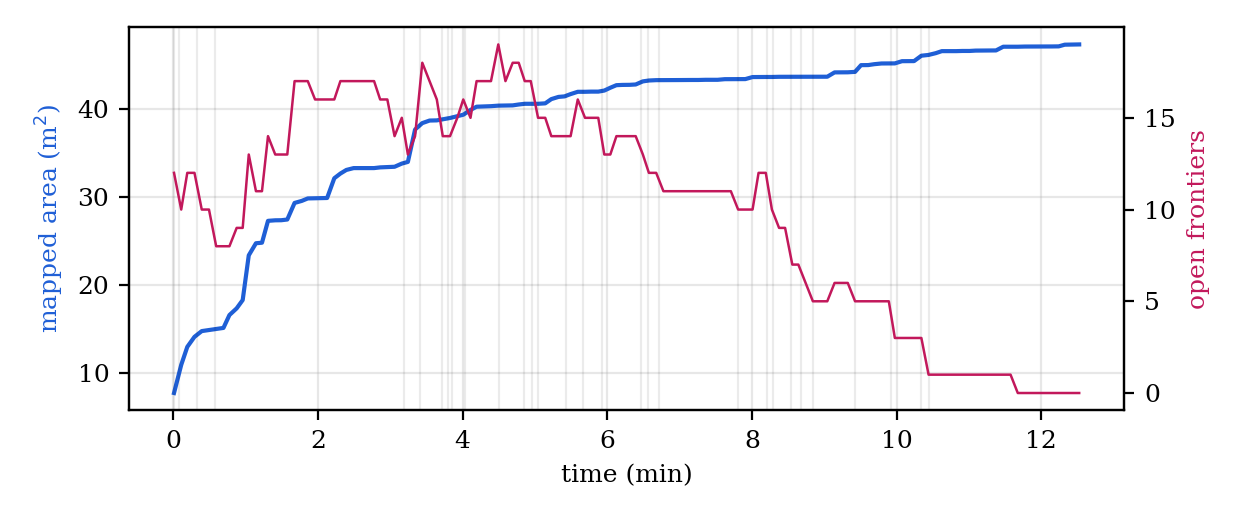
\includegraphics[width=\columnwidth]{figures/run_progress.png}
\caption{Mapped area (blue) and open frontiers (red) during the run; grey lines mark goals sent.}\label{fig:progress}
\end{figure}
